\documentclass[11pt]{amsart}
\usepackage[T1]{fontenc}
\usepackage{lmodern}
\usepackage{amsmath,amssymb,mathtools}
\usepackage{booktabs}
\usepackage{array}
\usepackage{tikz}
\usepackage{xcolor}
\usepackage{hyperref}
\hypersetup{colorlinks=true,linkcolor=blue!55!black,citecolor=blue!55!black,urlcolor=blue!55!black}

\newtheorem{theorem}{Theorem}[section]
\newtheorem{lemma}[theorem]{Lemma}
\newtheorem{proposition}[theorem]{Proposition}
\newtheorem{corollary}[theorem]{Corollary}
\theoremstyle{definition}
\newtheorem{definition}[theorem]{Definition}
\newtheorem{remark}[theorem]{Remark}

\newcommand{\R}{\mathbb{R}}
\newcommand{\Ftwo}{\mathbb{F}_2}
\newcommand{\len}{\operatorname{len}}
\newcommand{\dist}{\operatorname{dist}}
\newcommand{\DraftLabel}{\textcolor{red!70!black}{\bfseries DRAFT --- NOT YET EXTERNALLY PEER REVIEWED}}

\title[OPG-500 eight-vertex counterexample]{An Eight-Vertex Counterexample to OPG-500 on Geodesic Nonperipheral Cycles}
\author{[AUTHOR NAMES --- TO BE SUPPLIED]}
\address{[AFFILIATIONS AND POSTAL ADDRESSES --- TO BE SUPPLIED]}
\email{[PUBLIC EMAILS --- TO BE SUPPLIED]}
\thanks{ORCID, grants, acknowledgements, contribution statement, and approved AI/tool disclosure: [TO BE SUPPLIED].}
\date{Draft of 9 September 2026}
\subjclass[2020]{Primary 05C38 (provisional; official-code confirmation pending)}
\keywords{geodesic cycle, peripheral cycle, cycle space, weighted graph, formal verification}
\markboth{OPG-500 COUNTEREXAMPLE --- DRAFT}{OPG-500 COUNTEREXAMPLE --- DRAFT}
\emergencystretch=3em

\begin{document}

\begin{abstract}
We present a fixed simple graph $H$ with eight vertices and eighteen edges such that every strictly positive real edge weighting of $H$ admits a geodesic nonperipheral cycle.  Thus $H$ is a counterexample to the universal assertion in OPG-500 under the audited formulation used here.  The proof passes to the spanning subgraph of tight edges.  Assuming that every geodesic cycle is peripheral forces a triangle-free four-vertex tight core and four dominating tight links.  A finite counting inequality then puts all possible peripheral cycle vectors in a subspace whose dimension is smaller than the cycle rank.  A cycle outside that subspace can be chosen geodesic because positive-weight geodesic cycles generate the finite cycle space, yielding a contradiction.  We give the complete edge list, a conventional proof, and a declaration-level crosswalk to an accepted Lean theorem and an exact-toolchain replay.  Repository-level trusted Result admission and external peer review remain pending.
\end{abstract}

\maketitle
\begin{center}\DraftLabel\end{center}

\section{Introduction}

Open Problem Garden asks \cite{OPG500}:
\begin{quote}
If $G$ is a $3$-connected finite graph, is there an assignment of lengths $\ell:E(G)\to\mathbb R^+$ to the edges of $G$, such that every $\ell$-geodesic cycle is peripheral?
\end{quote}
Here a cycle is $\ell$-geodesic when no path between two of its vertices is shorter than both cycle arcs between those vertices.  A peripheral cycle is an induced nonseparating cycle.  Georgakopoulos and Spr\"ussel proved that, in a finite graph with positive edge lengths, every cycle is a mod-$2$ sum of geodetic cycles no longer than it \cite[Theorem~3.1]{GeorgakopoulosSpruessel2009}.  The question was motivated by Tutte's theorem that peripheral cycles generate the cycle space of a finite $3$-connected graph \cite{Tutte1963}; see also the accessible formulation in \cite[Theorem~1.3]{Kelmans2006}.

We use the canonical strict-positive interpretation $\mathbb R^+=\mathbb R_{>0}$.  The statement-faithfulness audit in Section~\ref{sec:verification} records that interpretation explicitly rather than silently broadening the source.

Our main result is the following.

\begin{theorem}[Main theorem]\label{thm:main}
There is a fixed finite simple graph $H$ on eight vertices and eighteen edges such that, for every function $\ell:E(H)\to\mathbb R_{>0}$, the weighted graph $(H,\ell)$ contains a cycle that is both $\ell$-geodesic and nonperipheral.
\end{theorem}

The proof is not a finite sampling of weights.  It handles an arbitrary positive-real assignment by constructing its tight-edge graph and deriving a dimension contradiction.  Section~\ref{sec:definitions} fixes conventions; Section~\ref{sec:graph} gives $H$; Section~\ref{sec:proof} proves the theorem; Section~\ref{sec:verification} states the formal and source boundaries.

\section{Definitions and notation}\label{sec:definitions}

All graphs are finite, undirected, loopless, and without parallel edges.  For a graph $G$, an \emph{edge weighting} is a function $\ell:E(G)\to\mathbb R$.  It is \emph{positive} if $\ell(e)>0$ for every edge $e$.  The length $\len_\ell(P)$ of a walk or path is the sum of its edge weights, with multiplicity for a walk.  For vertices $x,y$, $\dist_\ell(x,y)$ is the minimum length of a simple $x$--$y$ path.  The minimum exists because $G$ is finite.  A shortest path is always understood to be simple.

\begin{definition}\label{def:geodesic}
A simple cycle $C$ is \emph{$\ell$-geodesic} if, for every $x,y\in V(C)$, at least one of the two $x$--$y$ arcs of $C$ has length $\dist_\ell(x,y)$.  Equivalently, there is a globally shortest simple $x$--$y$ path whose edges lie in $C$.
\end{definition}

The equivalence includes ties.  For $x=y$, the zero-edge path supplies the formal witness.  Strict positivity ensures that deleting repeated portions of a walk does not increase its length and that every nontrivial path has positive length.

\begin{definition}\label{def:peripheral}
A cycle $C$ is \emph{peripheral} if it is chordless and $G-V(C)$ is connected or empty.  Otherwise it is \emph{nonperipheral}.
\end{definition}

A graph is \emph{$3$-connected} if it has at least four vertices and deleting any set of fewer than three vertices leaves a connected graph.  For a cycle $C$, let $\chi_C\in\Ftwo^{E(G)}$ denote its edge-incidence vector.  The cycle space is the span of these vectors, with addition given by symmetric difference.

An edge $xy$ is \emph{tight} for $\ell$ if its one-edge path is a globally shortest $x$--$y$ path.  The \emph{tight graph} $T=T(G,\ell)$ is the spanning subgraph containing exactly the tight edges, with the inherited weights.

\section{The eight-vertex graph}\label{sec:graph}

Let the core be $K=\{0,1,2,3\}$ and put $A=\{4,5,6,7\}$.  The graph $H$ has edge set
\begin{equation}\label{eq:edges}
\begin{split}
E(H)=\{&01,02,03,04,05,06,12,13,14,15,17,\\
       &23,24,26,27,35,36,37\}.
\end{split}
\end{equation}
Thus $K$ induces $K_4$, while $A$ is independent.  Vertex $4$ is adjacent to all core vertices except $3$; vertices $5,6,7$ miss core vertices $2,1,0$, respectively.

\begin{figure}[ht]
\centering
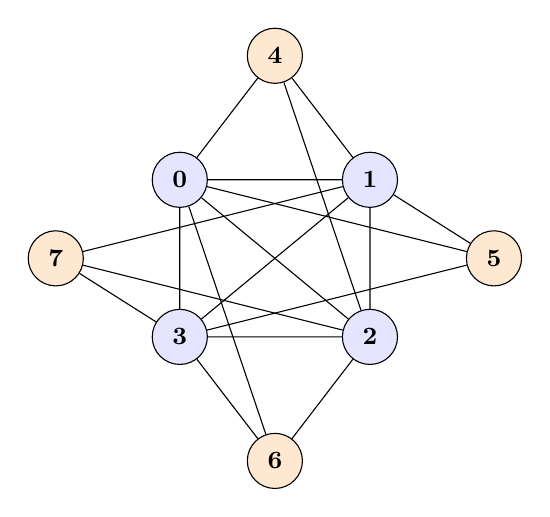
\begin{tikzpicture}[scale=1.05,
  core/.style={circle,draw=black,fill=blue!10,minimum size=7mm,inner sep=0pt,font=\small\bfseries},
  apex/.style={circle,draw=black,fill=orange!18,minimum size=7mm,inner sep=0pt,font=\small\bfseries},
  every edge/.style={draw=black!72,line width=.55pt}]
  \node[core] (v0) at (-1.15, 0.95) {0};
  \node[core] (v1) at ( 1.15, 0.95) {1};
  \node[core] (v2) at ( 1.15,-0.95) {2};
  \node[core] (v3) at (-1.15,-0.95) {3};
  \node[apex] (v4) at ( 0.00, 2.45) {4};
  \node[apex] (v5) at ( 2.65, 0.00) {5};
  \node[apex] (v6) at ( 0.00,-2.45) {6};
  \node[apex] (v7) at (-2.65, 0.00) {7};
  % Core K4: 01,02,03,12,13,23.
  \foreach \u/\v in {0/1,0/2,0/3,1/2,1/3,2/3}
    \draw (v\u) -- (v\v);
  % Apex 4 misses core 3; apex 5 misses 2; apex 6 misses 1; apex 7 misses 0.
  \foreach \u/\v in {4/0,4/1,4/2,5/0,5/1,5/3,6/0,6/2,6/3,7/1,7/2,7/3}
    \draw (v\u) -- (v\v);
\end{tikzpicture}

\caption{The graph $H$.  Blue vertices form the core $K_4$; orange vertices are independent.  The edge list \eqref{eq:edges}, not the drawing, is authoritative.}\label{fig:H}
\end{figure}

\begin{proposition}[Structure of $H$]\label{prop:structure}
The graph $H$ is $3$-connected.  Its peripheral cycles are exactly the following twelve triangles:
\begin{equation}\label{eq:peripheral}
\begin{gathered}
014,015,024,026,035,036,124,127,\
135,137,236,237.
\end{gathered}
\end{equation}
\end{proposition}

\begin{proof}
After deletion of at most two vertices, at least two core vertices remain and they are adjacent.  Every remaining vertex of $A$ misses only one core vertex, so it is adjacent to at least one remaining core vertex.  Hence the remaining graph is connected.

For the cycle classification, observe first that $A$ is independent and $K$ is complete.  A chordless cycle containing at least three core vertices must be a core triangle: any longer cycle has a core chord.  A chordless cycle containing exactly two core vertices must be a triangle containing one vertex of $A$; with two apex vertices, the edge between the two core vertices is a chord.  A cycle with fewer than two core vertices is impossible.  Consequently every chordless cycle is either a core triangle or an apex--core--core triangle.

A core triangle is separating.  If $k$ is the fourth core vertex, then the apex that misses $k$ has all three neighbors in the deleted triangle and becomes isolated.  Conversely, delete an apex and two of its three core neighbors.  The two remaining core vertices are adjacent, and every remaining apex is adjacent to at least one of them; the complement is connected.  There are $4\binom32=12$ such triangles, precisely those in \eqref{eq:peripheral}.
\end{proof}

The independent enumeration in the supplement checks the same edge count, degree sequence, deletion connectivity, and list \eqref{eq:peripheral} without using Figure~\ref{fig:H}.

\section{Proof architecture and proof of the main theorem}\label{sec:proof}

\subsection{Metric lemmas and geodesic generation}

\begin{lemma}[Tight-edge bridge]\label{lem:tightbridge}
Let $G$ be a finite connected graph with positive edge weighting $\ell$, and let $T=T(G,\ell)$.
\begin{enumerate}
\item Every two vertices are joined by a shortest path all of whose edges are tight; in particular, $T$ is connected.
\item If a cycle is geodesic in $T$ for the inherited weighting, then its image in $G$ is geodesic.
\item If $xy$ is not tight and $P$ is a shortest $x$--$y$ path, then $xy\cup P$ is a geodesic cycle, provided it is read as the simple cycle formed by the edge and the reverse of $P$.
\end{enumerate}
\end{lemma}

\begin{proof}
Choose a shortest simple path between any two vertices.  Every subpath of a shortest path is shortest: replacing a shorter middle segment and then removing repetitions would give a shorter path between the original endpoints.  In particular every one-edge subpath is tight, proving (1).

Lengths of walks in $T$ agree with lengths of their images in $G$.  Given a shortest path in $T$, compare it with a shortest path in $G$; by (1) the latter lifts to $T$.  It follows that a shortest path in $T$ remains shortest in $G$, proving (2).

For (3), the path $P$ cannot use $xy$, for then the one-edge subpath would be shortest and $xy$ would be tight.  Hence $xy\cup P$ is a simple cycle.  All its vertices lie on $P$, and the shortest subpath of $P$ between any two of them is supported in the cycle.  Thus the cycle is geodesic.
\end{proof}

\begin{theorem}[Finite weighted geodesic generation]\label{thm:generation}
Let $G$ be finite and let $\ell$ be positive.  Every cycle $C$ is a mod-$2$ sum of $\ell$-geodesic cycles, each of length at most $\len_\ell(C)$.
\end{theorem}

\begin{proof}
This is the finite theorem of Georgakopoulos and Spr\"ussel \cite[Theorem~3.1]{GeorgakopoulosSpruessel2009}; we include the strengthened descent argument formalized in the supplement.

Because $G$ has finitely many simple cycles, induction by weighted length is well founded on that finite set.  If $C$ is geodesic, there is nothing to prove.  Otherwise choose a bad pair $u,v\in V(C)$---one for which no shortest $u$--$v$ path is supported on $C$---and, among all bad pairs, choose a shortest path $P$ of minimum possible length.

The interior of $P$ is disjoint from $C$.  Indeed, if an internal vertex $w$ lay on $C$, both subpaths $uPw$ and $wPv$ would be shortest and would have strictly smaller positive length than $P$.  Minimality says that neither $(u,w)$ nor $(w,v)$ is bad, so shortest paths for both pairs can be chosen on $C$.  Concatenating them and deleting repetitions gives a shortest $u$--$v$ path on $C$, contradicting badness.  The same minimality/shortestness argument shows that no edge of $P$ lies on $C$.

Let $A$ and $B$ be the two $u$--$v$ arcs of $C$.  Since the pair is bad and $P$ is shortest,
\[
  \len_\ell(P)<\len_\ell(A),\qquad
  \len_\ell(P)<\len_\ell(B).
\]
The unions $C_1=P\cup A$ and $C_2=P\cup B$ are simple cycles, each strictly shorter than $C$, and
$\chi_{C_1}+\chi_{C_2}=\chi_C$ over $\Ftwo$.  Apply the induction hypothesis to $C_1$ and $C_2$.  Every resulting geodesic cycle is shorter than $C$ and their sum is $C$.
\end{proof}

\begin{lemma}[Geodesic outside a subspace]\label{lem:geooutside}
If a subspace $W\leq\Ftwo^{E(G)}$ misses some cycle vector, then for every positive weighting it misses the vector of some geodesic cycle.
\end{lemma}

\begin{proof}
Apply Theorem~\ref{thm:generation} to a cycle outside $W$.  If every geodesic summand belonged to $W$, then so would their sum.
\end{proof}

\subsection{The four-core obstruction}

Fix a positive weighting $\ell$ of $H$ and write $T=T(H,\ell)$.  Index the four apex vertices by $a_i=7-i$ for $i\in\{0,1,2,3\}$, so $a_i$ is adjacent to every core vertex except $i$.  Let $F=T[K]$ be the tight core.  Define
\[
 N_i=\{j\in K: a_i j\in E(T)\}.
\]
Thus $i\notin N_i$.

For the next lemmas, suppose toward a contradiction that
\begin{equation}\label{eq:hall}
  \text{every $\ell$-geodesic cycle of $H$ is peripheral.}
\end{equation}

\begin{lemma}[Two-step replacement]\label{lem:twostep}
Every non-tight edge $xy$ of $H$ has a two-edge replacement $xzy$ in $T$.
\end{lemma}

\begin{proof}
Take a shortest $x$--$y$ path $P$.  By Lemma~\ref{lem:tightbridge}, $xy\cup P$ is geodesic, hence peripheral by \eqref{eq:hall}.  Proposition~\ref{prop:structure} says every peripheral cycle has three vertices, so $P$ has exactly two edges.  Those edges are tight by the subpath property.
\end{proof}

\begin{lemma}[Core and links]\label{lem:corelinks}
The graph $F$ is triangle-free.  Moreover, for each $i$, the set $N_i$ dominates $K\setminus(\{i\}\cup N_i)$ in $F$: if $j\ne i$ and $j\notin N_i$, then some $k\in N_i$ satisfies $jk\in E(F)$.
\end{lemma}

\begin{proof}
If three core vertices formed a tight triangle, its three one-edge sides would witness geodesicity, but Proposition~\ref{prop:structure} says a core triangle is nonperipheral, contradicting \eqref{eq:hall}.

If $j\ne i$ and $j\notin N_i$, then $a_i j$ is an edge of $H$ but is not tight.  Lemma~\ref{lem:twostep} gives $a_i k j$ in $T$.  Every neighbor of $a_i$ is a core vertex $k\ne i$; hence $k\in N_i$ and $jk\in E(F)$.
\end{proof}

\begin{lemma}[Four-core rank gap]\label{lem:rankgap}
Let $F$ be any graph on $K=\{0,1,2,3\}$ and let $N_i\subseteq K\setminus\{i\}$ dominate the remaining vertices as in Lemma~\ref{lem:corelinks}.  If $c_i$ denotes the number of connected components of $F[N_i]$, then
\begin{equation}\label{eq:rankgap}
  7< |E(F)|+\sum_{i=0}^3 c_i.
\end{equation}
\end{lemma}

\begin{proof}
Let $A_i$ be the edges of $F$ internal to $N_i$, let $X_i=K\setminus(\{i\}\cup N_i)$, and let $B_i$ be the edges of $F-i$ crossing between $N_i$ and $X_i$.  Every graph on vertex set $N_i$ satisfies
$|N_i|\le c_i+|A_i|$.  Dominance allows us to choose, for every vertex of $X_i$, an incident edge to $N_i$; distinct vertices of $X_i$ give distinct crossing edges.  Therefore
\[
  3=|N_i|+|X_i|\le |N_i|+|B_i|.
\]
The disjoint sets $A_i$ and $B_i$ are contained in the edges of $F$ avoiding $i$, so
\[
 3\le c_i+|A_i|+|B_i|
   \le c_i+|E(F-i)|.
\]
Summing over $i$, and noting that every edge of a four-vertex graph avoids exactly two vertices, gives
\begin{equation}\label{eq:twelve}
  12\le \sum_i c_i+2|E(F)|.
\end{equation}
Each $N_i$ is nonempty: otherwise any $j\ne i$ would violate domination.  Hence $\sum_i c_i\ge4$.  The two integer inequalities imply $|E(F)|+\sum_i c_i\ge8$, which is \eqref{eq:rankgap}.
\end{proof}

Since $F$ is triangle-free and $|N_i|\le3$, each $F[N_i]$ is a forest.  If $q_i=|E(F[N_i])|$, then
\begin{equation}\label{eq:forest}
  q_i+c_i=|N_i|.
\end{equation}
Every edge of $T$ is either a core edge or an apex--core edge, so
\begin{equation}\label{eq:Tcount}
  |E(T)|=|E(F)|+\sum_i |N_i|.
\end{equation}
Combining \eqref{eq:rankgap}--\eqref{eq:Tcount} yields
\begin{equation}\label{eq:generatorgap}
  \sum_i q_i < |E(T)|+1-8.
\end{equation}

\subsection{Cycle vectors and the contradiction}

For every $i$ and every edge $jk$ of $F[N_i]$, the triangle $a_i j k$ lies in $T$.  Let $\mathcal S$ be the set of their edge vectors (viewed in $\Ftwo^{E(H)}$), and put $W=\operatorname{span}(\mathcal S)$.  Duplicates can only decrease cardinality, so by \eqref{eq:generatorgap}
\begin{equation}\label{eq:dimW}
 \dim W\le |\mathcal S|\le\sum_i q_i<|E(T)|+1-8.
\end{equation}

\begin{lemma}[Peripheral vectors lie in $W$]\label{lem:peripheralspan}
If a cycle of $T$ maps to a peripheral cycle of $H$, then its edge vector belongs to $W$.
\end{lemma}

\begin{proof}
By Proposition~\ref{prop:structure}, the image is one of the triangles $a_i j k$ in \eqref{eq:peripheral}.  Since all three of its edges lie in $T$, we have $j,k\in N_i$ and $jk\in E(F[N_i])$.  Its vector is therefore one of the generators in $\mathcal S$.
\end{proof}

The tight graph $T$ is connected by Lemma~\ref{lem:tightbridge}.  A connected graph on eight vertices has cycle-space dimension $|E(T)|-8+1$: choose a spanning tree and use the fundamental cycle of each non-tree edge.  Thus \eqref{eq:dimW} implies that some cycle vector of $T$ lies outside $W$.  By Lemma~\ref{lem:geooutside}, a cycle $C$ outside $W$ may be chosen geodesic for the inherited positive weighting.  Lemma~\ref{lem:tightbridge}(2) makes its image geodesic in $H$.  Assumption \eqref{eq:hall} would make that image peripheral, and Lemma~\ref{lem:peripheralspan} would put $\chi_C$ in $W$, a contradiction.  We have proved Theorem~\ref{thm:main}.

\begin{corollary}[Negative OPG-500 consequence]\label{cor:negative}
Under the audited finite-simple, strictly-positive-real, geodesic, and peripheral definitions of Section~\ref{sec:definitions}, the universal assertion posed by OPG-500 is false.
\end{corollary}

\begin{proof}
The assertion has logical form
\[
 \forall G\,[\,3\text{-connected}(G)\Rightarrow
   \exists\ell>0\;\forall C\,(C\text{ geodesic}\Rightarrow C\text{ peripheral})\,].
\]
Theorem~\ref{thm:main} supplies one $3$-connected $H$ for which every positive $\ell$ has a geodesic nonperipheral cycle, which is its direct negation.
\end{proof}

\section{Formal verification and statement faithfulness}\label{sec:verification}

The formal root declaration is
\begin{small}
\begin{verbatim}
OPG500Counterexample.eight_vertex_counterexample :
  IsThreeConnected H /\
    forall ell : EdgeWeight H, IsPositive ell ->
      exists C : Cycle H, C.IsGeodesic ell /\ not C.IsPeripheral
\end{verbatim}
\end{small}
(with ASCII notation shown here only for typesetting).  The fixed acceptance identity has status `Proved` and open leaves $0$:
\begin{center}\scriptsize\ttfamily
Theorem: 5c4997cd-9945-4028-b853-4ad91c324535\\
Submission: ed7c185a-9a49-4ded-90af-24839db25038\\
Accepted-root SHA-256: 30088256cdd8ed371c2d65d68688d4db7598be598ba401d3ac1a9d60d07267f6
\end{center}

A fresh bounded replay used the following pins:
\begin{center}\scriptsize\ttfamily
Lean 4.33.1: 819816b2e0a3bf405af45ae5c7af2491d8f5bee6\\
Lake: 5.0.0-src+819816b\\
Mathlib: 0df444a360eaa60ab8c11dca51a86af692955474
\end{center}
All five target modules exited $0$.  `\#print axioms` reported
\[
 [\texttt{propext},\ \texttt{Classical.choice},\ \texttt{Quot.sound}].
\]
This is not an assertion of axiom-freedom.  A separate nested-comment-aware source scan found no `sorry`, `admit`, custom `axiom`, `unsafe`, `extern`, `implemented\_by`, or `opaque` declaration in the accepted/replay scope.

\begin{table}[ht]
\centering\small
\caption{Statement-faithfulness summary.}\label{tab:faith}
\begin{tabular}{@{}p{.18\textwidth}p{.35\textwidth}p{.35\textwidth}@{}}
\toprule
Dimension & Source/contract & Formal theorem \\
\midrule
Domain & finite simple $3$-connected graphs & fixed `SimpleGraph (Fin 8)`, proved $3$-connected \\
Weights & $\mathbb R^+$; contract $\mathbb R_{>0}$ & all $\ell:E(H)\to\mathbb R$ with $0<\ell(e)$ \\
Geodesic & no path shorter than both arcs & a globally shortest simple path supported on the cycle \\
Peripheral & induced nonseparating & chordless, connected-or-empty deletion complement \\
Quantifiers & $\forall G\,\exists\ell\,\forall C$ & one $H$, then $\forall\ell\,\exists C$ with negated conclusion \\
Polarity & universal existence question & direct counterexample witness \\
\bottomrule
\end{tabular}
\end{table}

The source and formal geodesic definitions are equivalent in this finite positive setting: a shortest supported path is a cycle arc, while absence of a path shorter than both arcs forces the shorter arc to attain the finite minimum distance.  Tied shortest paths are allowed.  The graph precedes the weight quantifier, and the witness cycle may depend on the weighting.

The status boundary is essential:
\begin{quote}
The root mathematical statement has an accepted Lean proof and an exact-toolchain replay. The proof materials are public. Repository-level trusted Result admission and conventional external peer review are separate processes and are not implied by those facts.
\end{quote}

\section{Discussion}

The obstruction is not a special numerical weighting.  For each weighting, tight edges retain the ambient shortest-path metric.  If every geodesic cycle were peripheral, the finite peripheral classification would restrict all relevant cycle vectors to apex triangles.  The four-core inequality proves that these triangles are too few to span the tight graph's cycle space.  Geodesic generation then forces a geodesic cycle outside their span.

The result is limited to the definitions audited above.  It does not address zero or negative edge weights, infinite graphs, alternate notions of geodesicity or peripheral cycles, or stronger structural conclusions.  It does not show that eight vertices is minimal.  We make no claim of priority beyond the cited frozen materials, and no claim of external peer review.

\appendix
\section{Hand-check data}

The adjacency lists are
\[
\begin{array}{c|l}
0&1,2,3,4,5,6\\
1&0,2,3,4,5,7\\
2&0,1,3,4,6,7\\
3&0,1,2,5,6,7\\
4&0,1,2\\
5&0,1,3\\
6&0,2,3\\
7&1,2,3
\end{array}
\]
They give degree sequence $(6,6,6,6,3,3,3,3)$ and total degree $36$, hence eighteen edges.  The twelve peripheral triangles are listed in \eqref{eq:peripheral}.  The supplemental script exhaustively enumerates simple cycles and checks chordlessness and deletion connectivity.

\section{Paper--Lean crosswalk}

\begin{center}\small
\begin{tabular}{@{}ll@{}}
\toprule
Paper item & Lean declaration \\
\midrule
Proposition~\ref{prop:structure} & `OPG500Counterexample.eight\_vertex\_graph\_structure`\\
Lemma~\ref{lem:tightbridge} & `OPG500Counterexample.tight\_edge\_metric\_bridge`\\
Lemma~\ref{lem:twostep} & `OPG500Assembly.nontight\_twoStep`\\
Lemma~\ref{lem:corelinks} & `tightCore\_triangleFree`, `tightLinks\_dominates`\\
Lemma~\ref{lem:rankgap} & `OPG500Counterexample.core\_link\_rank\_gap`\\
Theorem~\ref{thm:generation} & `finite\_geodesic\_cycles\_generate`\\
Lemma~\ref{lem:geooutside} & `exists\_geodesic\_outside\_submodule`\\
Lemma~\ref{lem:peripheralspan} & `peripheral\_mapTightCycle\_mem\_span`\\
Theorem~\ref{thm:main} & `OPG500Counterexample.eight\_vertex\_counterexample`\\
\bottomrule
\end{tabular}
\end{center}
The complete machine-extracted declaration DAG and CSV crosswalk are `formal/theorem-dependency.json` and `formal/paper-lean-crosswalk.csv`.

\section{Replay and evidence manifest}

From the standalone replay directory (shown in reduced type to preserve exact module names):
\begin{scriptsize}
\begin{verbatim}
lake update
lake build Theorems.Thm_OPG500Counterexample_eight_vertex_graph_structure
lake build Theorems.Thm_OPG500Counterexample_tight_edge_metric_bridge
lake build Theorems.Thm_OPG500Counterexample_core_link_rank_gap
lake build Theorems.Thm_OPG500Counterexample_finite_geodesic_cycles_generate
lake build Theorems.Thm_OPG500Counterexample_eight_vertex_counterexample
\end{verbatim}
\end{scriptsize}
Commands, bounds, versions, exit codes, logs, source hashes, axiom output, and scans are recorded under `formal/`.  `publication-manifest.json` and `SHA256SUMS.txt` bind the complete draft bundle.  Admission templates under `evidence/admission-drafts/` are unsigned and remain pending trusted execution.

\bibliographystyle{amsplain}
\bibliography{references}

\end{document}
